\documentclass[11pt]{article}
\usepackage[a4paper,margin=1in]{geometry}
\usepackage{amsmath,amssymb,amsthm}
\usepackage{tikz}
\usepackage{booktabs}
\usepackage{xcolor}
\usepackage[hidelinks]{hyperref}
\hypersetup{pdftitle={Binary words with the same characteristic polynomial},pdfauthor={Vamshi Jandhyala}}
\setlength{\parskip}{0.4em}
\setlength{\parindent}{0pt}

\newtheorem{theorem}{Theorem}
\newtheorem{proposition}[theorem]{Proposition}
\newtheorem{lemma}[theorem]{Lemma}
\theoremstyle{remark}
\newtheorem*{remark}{Remark}

\definecolor{inkblue}{RGB}{40,76,105}
\definecolor{rust}{RGB}{173,80,45}
\definecolor{sage}{RGB}{96,140,90}
\definecolor{ink}{RGB}{70,70,70}
\definecolor{paper}{RGB}{246,244,238}

\newcommand{\T}{^{\mathsf T}}

\title{Binary words with the same characteristic polynomial: \\ a block-reversal lemma and a census to length 22}
\author{Vamshi Jandhyala}
\date{}

\begin{document}
\maketitle
\vspace{-2em}

\begin{abstract}
For a binary word $w$ let $H_w$ be the tridiagonal matrix with $w$ on the diagonal and ones beside it. Philip Weiss
asked on MathOverflow when two words that are not reverses of each other give the same characteristic polynomial. We
prove one lemma that covers every mechanism known so far: if a symmetric $2\times2$ matrix $G$ is compatible with the
transfer matrices of some blocks and with the context around them, the blocks can be put in reverse order without
changing the polynomial. Reversal itself, the interleaving family from an earlier answer and a new ratio-class family
are three cases. An exhaustive census to length $22$ finds $822$ classes of words with a common polynomial; all but
$17$ of them are explained by the lemma together with complementation, and $154$ of the pairs need a matrix $G$
outside both named families. We extend the count of distinct polynomials to $n=22$. The lemma and its two families
are checked in the Lean proof assistant.
\end{abstract}

\section{The question}

Write $H_w$ for the $n\times n$ matrix with the letters $w_1,\dots,w_n\in\{0,1\}$ on the diagonal, ones immediately
above and below it, and zeros elsewhere, and $P_w(t)=\det(tI-H_w)$ for its characteristic polynomial. Reading the
word backwards gives the same polynomial, since $H_{w^*}$ is $H_w$ with rows and columns in reverse order. Weiss
\cite{MO} counted the distinct polynomials,
\[
a_n=2,3,6,10,20,36,72,134,270,526,1052,2072,4154,8231,16504,\dots,
\]
observed that reversal is the only coincidence for $n\le7$, and asked for a formula for $a_n$ and for a description of
the other coincidences. The smallest ones occur at $n=8$. Here is one of them:
\[
P_{10110010}=P_{10010110}.
\]
Stop and look for the reason before reading on. Both words start and end with $10$ and contain $10$ three times; what
changes is the order of the two letters between the copies.

An earlier answer to the question \cite{MOans} explains this example and a whole family like it. Our aim is a single
statement that explains it together with every other coincidence we can find, and an honest list of the ones it does
not explain.

\section{Transfer matrices}

Expanding $\det(tI-H_w)$ along its last row gives the three-term recurrence
\[
P_{wcd}=(t-d)\,P_{wc}-P_w ,\qquad P_\varnothing=1,\quad P_c=t-c ,
\]
for letters $c,d$, which is the recurrence of a continuant \cite[\S6.7]{GKP}. It packages into $2\times2$ matrices. Put
\[
T(z)=\begin{pmatrix} z&-1\\ 1&0\end{pmatrix},\qquad M_w=T(t-w_1)\,T(t-w_2)\cdots T(t-w_n),\qquad e=\begin{pmatrix}1\\0\end{pmatrix}.
\]
Then $P_w$ is the top-left entry of $M_w$, that is $P_w=e\T M_w e$, because the top row of $M_wT(t-c)$ is the top row
of $M_w$ pushed through the recurrence. Each $T(z)$ has determinant $1$, so $\det M_w=1$. We write the entries as
\[
M_w=\begin{pmatrix} p&-\rho\\ q&-s\end{pmatrix};
\]
here $p=P_w$, and $q$, $\rho$, $s$ are the polynomials of $w$ with its first letter, its last letter, or both removed
(as noted in~\cite{MOans}; we use only the entries).

The point of the matrices is that concatenation becomes multiplication: $M_{AVB}=M_AM_VM_B$, so
\begin{equation}\label{eq:split}
P_{AVB}=x_A\T\, M_V\, y_B ,\qquad x_A=M_A\T e,\quad y_B=M_Be .
\end{equation}
Read this as: the context $A$ and $B$ enters only through two vectors, and the middle $V$ only through its matrix.

Reversal is already an instance of what follows. Let $D=\operatorname{diag}(1,-1)$. Then
$T(z)D=\left(\begin{smallmatrix} z&1\\1&0\end{smallmatrix}\right)$ is symmetric, that is $T(z)D=DT(z)\T$, and
transposing $P_w=e\T M_we$ moves $D$ through the product one letter at a time, which reverses the word.

\section{The block-reversal lemma}

\begin{lemma}\label{lem:block}
Let $G$ be a symmetric $2\times2$ matrix over a commutative ring, let $N_1,\dots,N_m$ be $2\times2$ matrices with
$N_iG=GN_i\T$ for every $i$, and let $x,x',y,y'$ be vectors and $\lambda,\lambda'$ scalars with
\[
Gx=\lambda y',\qquad Gx'=\lambda' y .
\]
Then $\lambda'\,x\T N_1\cdots N_m\,y=\lambda\,x'^{\mathsf T} N_m\cdots N_1\,y'$.
\end{lemma}

\begin{proof}
Write $V=N_1\cdots N_m$ and $V_{\rm rev}=N_m\cdots N_1$. Moving $G$ across one factor at a time gives
$GV\T=GN_m\T\cdots N_1\T=N_mGN_{m-1}\T\cdots N_1\T=\dots=V_{\rm rev}G$. Hence
\[
\lambda'\,x\T Vy=x\T VGx'=x'^{\mathsf T}(VG)\T x=x'^{\mathsf T}GV\T x=x'^{\mathsf T}V_{\rm rev}Gx=\lambda\,x'^{\mathsf T}V_{\rm rev}y' ,
\]
where the second step transposes a scalar and the third uses $G\T=G$.
\end{proof}

The condition $NG=GN\T$ says that $NG$ is symmetric. For $N=M_Y$ with entries $p',q',\rho',s'$ and
$G=\left(\begin{smallmatrix}\alpha&\beta\\ \beta&\gamma\end{smallmatrix}\right)$ it is one linear equation,
\begin{equation}\label{eq:lin}
q'\alpha-(p'+s')\beta+\rho'\gamma=0 ,
\end{equation}
and each condition $Gx\parallel y'$ is linear in $G$ as well. So, for given words, whether a suitable $G$ exists is a
question of linear algebra over $\mathbb{Q}(t)$.

Combining the lemma with~\eqref{eq:split}, for words $A,A',B,B'$ and blocks $Y_1,\dots,Y_m$:

\begin{theorem}\label{thm:words}
If $G\T=G$, $M_{Y_i}G$ is symmetric for every $i$, $Gx_A=\lambda y_{B'}$ and $Gx_{A'}=\lambda y_B$ with
$\lambda\ne0$ in $\mathbb{Z}[t]$, then $P_{A\,Y_1\cdots Y_m\,B}=P_{A'\,Y_m\cdots Y_1\,B'}$.
\end{theorem}

Figure~\ref{fig:blocks} shows three examples, one for each of the families below.

\begin{figure}[ht]
\centering
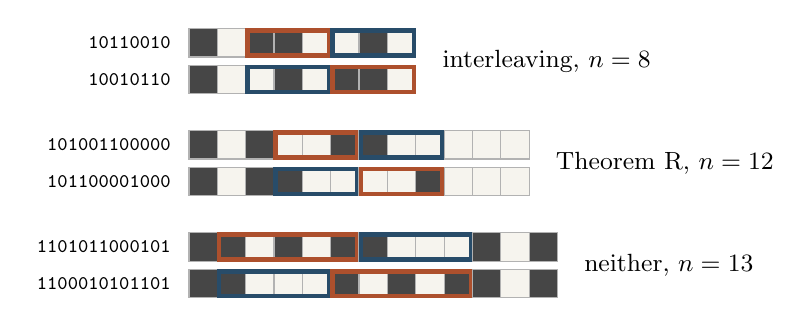
\begin{tikzpicture}[x=0.36cm,y=0.36cm]
  \fill[ink] (0,0) rectangle ++(1,1);
  \draw[gray!60] (0,0) rectangle ++(1,1);
  \fill[paper] (1,0) rectangle ++(1,1);
  \draw[gray!60] (1,0) rectangle ++(1,1);
  \fill[ink] (2,0) rectangle ++(1,1);
  \draw[gray!60] (2,0) rectangle ++(1,1);
  \fill[ink] (3,0) rectangle ++(1,1);
  \draw[gray!60] (3,0) rectangle ++(1,1);
  \fill[paper] (4,0) rectangle ++(1,1);
  \draw[gray!60] (4,0) rectangle ++(1,1);
  \draw[rust,line width=1.6pt] (2+0.06,0+0.06) rectangle (5-0.06,0+0.94);
  \fill[paper] (5,0) rectangle ++(1,1);
  \draw[gray!60] (5,0) rectangle ++(1,1);
  \fill[ink] (6,0) rectangle ++(1,1);
  \draw[gray!60] (6,0) rectangle ++(1,1);
  \fill[paper] (7,0) rectangle ++(1,1);
  \draw[gray!60] (7,0) rectangle ++(1,1);
  \draw[inkblue,line width=1.6pt] (5+0.06,0+0.06) rectangle (8-0.06,0+0.94);
  \fill[ink] (0,-1.3) rectangle ++(1,1);
  \draw[gray!60] (0,-1.3) rectangle ++(1,1);
  \fill[paper] (1,-1.3) rectangle ++(1,1);
  \draw[gray!60] (1,-1.3) rectangle ++(1,1);
  \fill[paper] (2,-1.3) rectangle ++(1,1);
  \draw[gray!60] (2,-1.3) rectangle ++(1,1);
  \fill[ink] (3,-1.3) rectangle ++(1,1);
  \draw[gray!60] (3,-1.3) rectangle ++(1,1);
  \fill[paper] (4,-1.3) rectangle ++(1,1);
  \draw[gray!60] (4,-1.3) rectangle ++(1,1);
  \draw[inkblue,line width=1.6pt] (2+0.06,-1.3+0.06) rectangle (5-0.06,-1.3+0.94);
  \fill[ink] (5,-1.3) rectangle ++(1,1);
  \draw[gray!60] (5,-1.3) rectangle ++(1,1);
  \fill[ink] (6,-1.3) rectangle ++(1,1);
  \draw[gray!60] (6,-1.3) rectangle ++(1,1);
  \fill[paper] (7,-1.3) rectangle ++(1,1);
  \draw[gray!60] (7,-1.3) rectangle ++(1,1);
  \draw[rust,line width=1.6pt] (5+0.06,-1.3+0.06) rectangle (8-0.06,-1.3+0.94);
  \node[right,font=\small] at (8.6,-0.15) {interleaving, $n=8$};
  \node[left,font=\scriptsize\ttfamily] at (-0.3,0.5) {10110010};
  \node[left,font=\scriptsize\ttfamily] at (-0.3,-0.8) {10010110};
  \fill[ink] (0,-3.6) rectangle ++(1,1);
  \draw[gray!60] (0,-3.6) rectangle ++(1,1);
  \fill[paper] (1,-3.6) rectangle ++(1,1);
  \draw[gray!60] (1,-3.6) rectangle ++(1,1);
  \fill[ink] (2,-3.6) rectangle ++(1,1);
  \draw[gray!60] (2,-3.6) rectangle ++(1,1);
  \fill[paper] (3,-3.6) rectangle ++(1,1);
  \draw[gray!60] (3,-3.6) rectangle ++(1,1);
  \fill[paper] (4,-3.6) rectangle ++(1,1);
  \draw[gray!60] (4,-3.6) rectangle ++(1,1);
  \fill[ink] (5,-3.6) rectangle ++(1,1);
  \draw[gray!60] (5,-3.6) rectangle ++(1,1);
  \draw[rust,line width=1.6pt] (3+0.06,-3.6+0.06) rectangle (6-0.06,-3.6+0.94);
  \fill[ink] (6,-3.6) rectangle ++(1,1);
  \draw[gray!60] (6,-3.6) rectangle ++(1,1);
  \fill[paper] (7,-3.6) rectangle ++(1,1);
  \draw[gray!60] (7,-3.6) rectangle ++(1,1);
  \fill[paper] (8,-3.6) rectangle ++(1,1);
  \draw[gray!60] (8,-3.6) rectangle ++(1,1);
  \draw[inkblue,line width=1.6pt] (6+0.06,-3.6+0.06) rectangle (9-0.06,-3.6+0.94);
  \fill[paper] (9,-3.6) rectangle ++(1,1);
  \draw[gray!60] (9,-3.6) rectangle ++(1,1);
  \fill[paper] (10,-3.6) rectangle ++(1,1);
  \draw[gray!60] (10,-3.6) rectangle ++(1,1);
  \fill[paper] (11,-3.6) rectangle ++(1,1);
  \draw[gray!60] (11,-3.6) rectangle ++(1,1);
  \fill[ink] (0,-4.9) rectangle ++(1,1);
  \draw[gray!60] (0,-4.9) rectangle ++(1,1);
  \fill[paper] (1,-4.9) rectangle ++(1,1);
  \draw[gray!60] (1,-4.9) rectangle ++(1,1);
  \fill[ink] (2,-4.9) rectangle ++(1,1);
  \draw[gray!60] (2,-4.9) rectangle ++(1,1);
  \fill[ink] (3,-4.9) rectangle ++(1,1);
  \draw[gray!60] (3,-4.9) rectangle ++(1,1);
  \fill[paper] (4,-4.9) rectangle ++(1,1);
  \draw[gray!60] (4,-4.9) rectangle ++(1,1);
  \fill[paper] (5,-4.9) rectangle ++(1,1);
  \draw[gray!60] (5,-4.9) rectangle ++(1,1);
  \draw[inkblue,line width=1.6pt] (3+0.06,-4.9+0.06) rectangle (6-0.06,-4.9+0.94);
  \fill[paper] (6,-4.9) rectangle ++(1,1);
  \draw[gray!60] (6,-4.9) rectangle ++(1,1);
  \fill[paper] (7,-4.9) rectangle ++(1,1);
  \draw[gray!60] (7,-4.9) rectangle ++(1,1);
  \fill[ink] (8,-4.9) rectangle ++(1,1);
  \draw[gray!60] (8,-4.9) rectangle ++(1,1);
  \draw[rust,line width=1.6pt] (6+0.06,-4.9+0.06) rectangle (9-0.06,-4.9+0.94);
  \fill[paper] (9,-4.9) rectangle ++(1,1);
  \draw[gray!60] (9,-4.9) rectangle ++(1,1);
  \fill[paper] (10,-4.9) rectangle ++(1,1);
  \draw[gray!60] (10,-4.9) rectangle ++(1,1);
  \fill[paper] (11,-4.9) rectangle ++(1,1);
  \draw[gray!60] (11,-4.9) rectangle ++(1,1);
  \node[right,font=\small] at (12.6,-3.75) {Theorem R, $n=12$};
  \node[left,font=\scriptsize\ttfamily] at (-0.3,-3.1) {101001100000};
  \node[left,font=\scriptsize\ttfamily] at (-0.3,-4.4) {101100001000};
  \fill[ink] (0,-7.2) rectangle ++(1,1);
  \draw[gray!60] (0,-7.2) rectangle ++(1,1);
  \fill[ink] (1,-7.2) rectangle ++(1,1);
  \draw[gray!60] (1,-7.2) rectangle ++(1,1);
  \fill[paper] (2,-7.2) rectangle ++(1,1);
  \draw[gray!60] (2,-7.2) rectangle ++(1,1);
  \fill[ink] (3,-7.2) rectangle ++(1,1);
  \draw[gray!60] (3,-7.2) rectangle ++(1,1);
  \fill[paper] (4,-7.2) rectangle ++(1,1);
  \draw[gray!60] (4,-7.2) rectangle ++(1,1);
  \fill[ink] (5,-7.2) rectangle ++(1,1);
  \draw[gray!60] (5,-7.2) rectangle ++(1,1);
  \draw[rust,line width=1.6pt] (1+0.06,-7.2+0.06) rectangle (6-0.06,-7.2+0.94);
  \fill[ink] (6,-7.2) rectangle ++(1,1);
  \draw[gray!60] (6,-7.2) rectangle ++(1,1);
  \fill[paper] (7,-7.2) rectangle ++(1,1);
  \draw[gray!60] (7,-7.2) rectangle ++(1,1);
  \fill[paper] (8,-7.2) rectangle ++(1,1);
  \draw[gray!60] (8,-7.2) rectangle ++(1,1);
  \fill[paper] (9,-7.2) rectangle ++(1,1);
  \draw[gray!60] (9,-7.2) rectangle ++(1,1);
  \draw[inkblue,line width=1.6pt] (6+0.06,-7.2+0.06) rectangle (10-0.06,-7.2+0.94);
  \fill[ink] (10,-7.2) rectangle ++(1,1);
  \draw[gray!60] (10,-7.2) rectangle ++(1,1);
  \fill[paper] (11,-7.2) rectangle ++(1,1);
  \draw[gray!60] (11,-7.2) rectangle ++(1,1);
  \fill[ink] (12,-7.2) rectangle ++(1,1);
  \draw[gray!60] (12,-7.2) rectangle ++(1,1);
  \fill[ink] (0,-8.5) rectangle ++(1,1);
  \draw[gray!60] (0,-8.5) rectangle ++(1,1);
  \fill[ink] (1,-8.5) rectangle ++(1,1);
  \draw[gray!60] (1,-8.5) rectangle ++(1,1);
  \fill[paper] (2,-8.5) rectangle ++(1,1);
  \draw[gray!60] (2,-8.5) rectangle ++(1,1);
  \fill[paper] (3,-8.5) rectangle ++(1,1);
  \draw[gray!60] (3,-8.5) rectangle ++(1,1);
  \fill[paper] (4,-8.5) rectangle ++(1,1);
  \draw[gray!60] (4,-8.5) rectangle ++(1,1);
  \draw[inkblue,line width=1.6pt] (1+0.06,-8.5+0.06) rectangle (5-0.06,-8.5+0.94);
  \fill[ink] (5,-8.5) rectangle ++(1,1);
  \draw[gray!60] (5,-8.5) rectangle ++(1,1);
  \fill[paper] (6,-8.5) rectangle ++(1,1);
  \draw[gray!60] (6,-8.5) rectangle ++(1,1);
  \fill[ink] (7,-8.5) rectangle ++(1,1);
  \draw[gray!60] (7,-8.5) rectangle ++(1,1);
  \fill[paper] (8,-8.5) rectangle ++(1,1);
  \draw[gray!60] (8,-8.5) rectangle ++(1,1);
  \fill[ink] (9,-8.5) rectangle ++(1,1);
  \draw[gray!60] (9,-8.5) rectangle ++(1,1);
  \draw[rust,line width=1.6pt] (5+0.06,-8.5+0.06) rectangle (10-0.06,-8.5+0.94);
  \fill[ink] (10,-8.5) rectangle ++(1,1);
  \draw[gray!60] (10,-8.5) rectangle ++(1,1);
  \fill[paper] (11,-8.5) rectangle ++(1,1);
  \draw[gray!60] (11,-8.5) rectangle ++(1,1);
  \fill[ink] (12,-8.5) rectangle ++(1,1);
  \draw[gray!60] (12,-8.5) rectangle ++(1,1);
  \node[right,font=\small] at (13.6,-7.3500000000000005) {neither, $n=13$};
  \node[left,font=\scriptsize\ttfamily] at (-0.3,-6.7) {1101011000101};
  \node[left,font=\scriptsize\ttfamily] at (-0.3,-8.0) {1100010101101};
\end{tikzpicture}

\caption{Three block reversals. Dark cells are $1$, light cells $0$; each block keeps its frame colour when the
blocks are put in reverse order. In each pair the two words have the same characteristic polynomial and are not
reverses of each other.}
\label{fig:blocks}
\end{figure}

\section{Three families}

\paragraph{Interleaving.} Fix a word $W$ with entries $p,q,\rho,s$ and letters $a_1,\dots,a_r$. The earlier
answer~\cite{MOans} shows that $P_{Wa_1Wa_2\cdots Wa_rW}$ depends on the letters only up to reversal.

\begin{proposition}\label{prop:inter}
$P_{W a_1W\cdots a_rW}=P_{Wa_rW\cdots a_1W}$. In Theorem~\ref{thm:words} take $A=A'=W$, blocks $a_iW$, empty $B$,
\[
G=\begin{pmatrix}1-\rho^2&-\rho p\\-\rho p&-p^2\end{pmatrix},\qquad \lambda=p .
\]
\end{proposition}

\begin{proof}
With $x_A=(p,-\rho)\T$ one finds $Gx_A=(p,0)\T=p\,e=p\,y_B$. For a block, $M_{aW}=T(t-a)M_W$ has entries
$p'=(t-a)p-q$, $q'=p$, $\rho'=(t-a)\rho-s$ and $s'=\rho$. Substituting into~\eqref{eq:lin}, the terms in $t-a$ cancel
and the left side becomes $p\,\bigl(1-(q\rho-ps)\bigr)=p\,(1-\det M_W)=0$. Finally $p=P_W$ is monic, so
$\lambda\neq0$.
\end{proof}

At $n=8$ this is the example from the introduction: $W=10$ and the letters $1,0$ become $0,1$.

\paragraph{The ratio class.} For a word $Y$ with entries $p',q',\rho',s'$ put $\kappa(Y)=(q'+\rho')/(p'+s')$.

\begin{proposition}[Theorem R]\label{prop:R}
Let $X$ be a word whose first letter $c$ differs from its last letter, with entries $p,q,\rho,s$ and $h=q+\rho$. Let
$A$ be $X$ with its first letter flipped and $B$ be $X$ with its last letter flipped. If $\kappa(Y_i)=\kappa(X)$ for
every $i$ (for instance $Y_i\in\{X,X^*\}$), then $P_{A\,Y_1\cdots Y_m\,B}=P_{A\,Y_m\cdots Y_1\,B}$.
\end{proposition}

\begin{proof}
Take $G=\left(\begin{smallmatrix}p+s&h\\ h&p+s\end{smallmatrix}\right)$. By~\eqref{eq:lin}, $M_YG$ is symmetric exactly
when $(q'+\rho')(p+s)=(p'+s')h$, which is $\kappa(Y)=\kappa(X)$; in particular it holds for $Y=X$. Let $\varepsilon=1$
if $c=1$ and $\varepsilon=-1$ if $c=0$, and $u=(1,\varepsilon)\T$. Flipping the first letter changes $T(t-c)$ to
$T(t-c)+\varepsilon\,ee\T$, and since $e\T=(0,1)\,T(z)$ for every $z$, this gives $x_A=M_X\T u$. In the same way,
flipping the last letter gives $y_B=M_Xu$. Now $Gu=(p+s+\varepsilon h)\,u$, so
\[
Gx_A=GM_X\T u=M_XGu=(p+s+\varepsilon h)\,y_B ,
\]
using $M_XG=GM_X\T$. Theorem~\ref{thm:words} applies with $A'=A$, $B'=B$ and $\lambda=p+s+\varepsilon h$, which is
monic of degree $|X|$ because $p$ is and the other entries have smaller degree.
\end{proof}

The first instances are at $n=12$: with $X=001$, $A=101$, $B=000$ and blocks $001$, $100$,
\[
P_{101\,001\,100\,000}=P_{101\,100\,001\,000}.
\]
The hypothesis on the end letters matters. If $X$ starts and ends with the same letter, flipping the two ends gives
the vectors $(1,\varepsilon)$ and $(1,-\varepsilon)$, which are different eigenvectors of $G$, and the argument fails;
in random trials the identity then fails every time.

\paragraph{Complementation.} Swapping $0$ and $1$ is not a reversal, but it relates polynomials in a simple way:
$P_{\overline w}(t)=(-1)^nP_w(1-t)$, as the earlier answer notes. The proof is one line:
$T(t-\bar c)=-D\,T\bigl((1-t)-c\bigr)D$ and $D^2=I$. So $\overline w$ shares the polynomial of $w$ whenever $P_w$ is
symmetric under $t\mapsto1-t$ (up to sign). The question's own example $00011011$, $00100111$ is of this kind.

\paragraph{Beyond the named families.} Many coincidences need a $G$ of neither shape. The smallest are at $n=13$, for
instance
\[
P_{1\,10101\,1000\,101}=P_{1\,1000\,10101\,101},
\]
with $A=A'=1$, $B=B'=101$, $\lambda=t^4-3t^3+4t-1$ and
$G=\left(\begin{smallmatrix}\alpha&\beta\\ \beta&\gamma\end{smallmatrix}\right)$, where
\[
\alpha=(t^3-2t^2-t+1)(t^3-2t^2-t+3),\quad \beta=(t-1)(t^4-2t^3-2t^2+3t+1),\quad \gamma=t(t-2)(t^2-2).
\]
The same $G$ serves the blocks $10111$ and $1000$ in the same context, so the swap $1\,10111\,1000\,101\sim
1\,1000\,10111\,101$ holds as well.

\section{The census}

We enumerated all words of length $n\le22$, grouped them by polynomial (fingerprinted at two points modulo
$2^{61}-1$, then every group confirmed with exact integer polynomials), and counted the classes that contain more
than one reversal pair. For each class we joined two of its reversal pairs when one is the complement of the other,
or when some splitting of the two words and some $G$ satisfy Theorem~\ref{thm:words}. The conditions on $G$ are
linear, so the search solves them modulo a large prime at random values of $t$; every move it found was then
confirmed exactly over $\mathbb{Q}(t)$. A class counts as explained when its reversal pairs are all joined.

\begin{table}[ht]
\centering
\small
\begin{tabular}{rrrrr}
\toprule
$n$ & $a_n$ & excess $r_n-a_n$ & classes & unexplained \\
\midrule
8 & 134 & 2 & 2 & 0 \\
9 & 270 & 2 & 2 & 2 \\
10 & 526 & 2 & 2 & 0 \\
11 & 1\,052 & 4 & 4 & 0 \\
12 & 2\,072 & 8 & 8 & 0 \\
13 & 4\,154 & 6 & 6 & 2 \\
14 & 8\,231 & 25 & 25 & 0 \\
15 & 16\,504 & 8 & 8 & 0 \\
16 & 32\,856 & 40 & 40 & 0 \\
17 & 65\,764 & 28 & 28 & 2 \\
18 & 131\,249 & 79 & 78 & 1 \\
19 & 262\,604 & 52 & 52 & 4 \\
20 & 524\,606 & 194 & 194 & 2 \\
21 & 1\,049\,560 & 40 & 40 & 0 \\
22 & 2\,097\,843 & 333 & 333 & 4 \\
\bottomrule
\end{tabular}
\caption{Distinct polynomials $a_n$, the excess over the number $r_n=(2^n+2^{\lceil n/2\rceil})/2$ of words up to
reversal, the classes of reversal pairs with a common polynomial, and the classes not explained by complementation
and block reversal. Every class holds two reversal pairs except one at $n=18$, which holds three.}
\label{tab:census}
\end{table}

Table~\ref{tab:census} gives the result. The values of $a_n$ for $n\le15$ agree with Weiss's, and those for
$16\le n\le22$ are new; the sequence is not in the OEIS (searched 10 October 2026). Of the $822$ classes, $805$ are
explained. Counting pairs of reversal pairs joined by a block reversal, $123$ are interleavings, $56$ have a $G$ with
equal diagonal entries as in Theorem~R, and $154$ need some other $G$.

The excess stays small: $(r_n-a_n)/2^{n/2}$ lies between $0.02$ and $0.2$ for $8\le n\le22$, which suggests
$a_n=2^{n-1}+O(2^{n/2})$, but we have no proof.

\section{What is left}

Seventeen classes are not explained. The first is
\[
P_{111010100}=P_{100110110}\qquad(n=9),
\]
together with its complement $110101000\sim100100110$. Its polynomial is irreducible of degree~$9$, and no splitting
of the two words into context and blocks admits a $G$ as in Theorem~\ref{thm:words}. The others are at $n=13$, $17$,
$18$ (the class with three reversal pairs), $19$, $20$ and $22$. So the answer to Weiss's
second question is, as far as length $22$: complementation and block reversal, plus a sporadic remainder that
neither explains. Whether the remainder comes from a further mechanism, or the block-reversal lemma has a natural
generalisation that reaches it, is open, as is a formula for $a_n$.

\paragraph{Verification.} Lemma~\ref{lem:block}, Theorem~\ref{thm:words}, Propositions~\ref{prop:inter}
and~\ref{prop:R}, the complement identity, the recurrence for $P$ and the degree facts used to cancel $\lambda$ are
proved in Lean~4 with Mathlib~\cite{mathlib}, using only the standard axioms; there $P_w$ is defined as the top-left
entry of $M_w$, and its agreement with the determinant is the classical expansion quoted above. The census is a
computation: the enumeration, the exact confirmation of every class, the search for $G$ and the exact confirmation of
all $333$ moves it found are in Python and C, together with an exhaustive check for $n\le8$ that the search never
accepts a move between words with different polynomials, deliberately broken versions of each program, and an
independent program that recounts $a_n$ for $n\le18$ and redoes the census for $n\le16$
in exact rational arithmetic. Everything is at \url{https://github.com/jvvk/mathematics/tree/main/binary-word-polynomials}.

\paragraph{Acknowledgements.} Philip Weiss asked the question~\cite{MO}; the transfer matrices, the complement
identity and the interleaving family are in the answer by user590443~\cite{MOans}, and Kevin Costello's comments
there relate $P_w$ to closed walks on a path with loops. Anthropic's Claude (Opus~5.5) was used to run the
computations, write the Lean formalisation and the programs, and draft this text. The author takes responsibility for
the content.

\begin{thebibliography}{9}
\bibitem{MO} P.~Weiss, When do two binary strings have the same characteristic polynomial?, MathOverflow question
514920 (2026), \url{https://mathoverflow.net/q/514920}, accessed 10 October 2026.
\bibitem{MOans} user590443, answer to~\cite{MO}, MathOverflow answer 515106 (2026),
\url{https://mathoverflow.net/a/515106}, accessed 10 October 2026.
\bibitem{GKP} R.~L.~Graham, D.~E.~Knuth and O.~Patashnik, \emph{Concrete Mathematics}, 2nd ed., Addison-Wesley,
1994.
\bibitem{mathlib} The mathlib Community, The Lean mathematical library, in \emph{Proceedings of the 9th ACM
SIGPLAN International Conference on Certified Programs and Proofs (CPP 2020)}, 367--381,
\href{https://doi.org/10.1145/3372885.3373824}{doi:10.1145/3372885.3373824}.
\end{thebibliography}

\bigskip
\noindent Vamshi Jandhyala, London, UK.

\end{document}
